% ==============================================================================
% DOCUMENT HEADER
% ==============================================================================

\documentclass[11t, a4paper, twocolumn]{article} 
\usepackage[english]{babel}
\usepackage{microtype}
\usepackage{amsmath,amsfonts,amsthm}
\usepackage[svgnames]{xcolor}
\usepackage[hang, small, labelfont=bf, up, textfont=it]{caption}
\usepackage{booktabs}
\usepackage{lastpage}
\usepackage{graphicx}
\usepackage{enumitem}
\setlist{noitemsep}
\usepackage{sectsty}
\allsectionsfont{\usefont{OT1}{phv}{b}{n}}
\usepackage{lipsum}
\usepackage{geometry}
\geometry{
	top=1cm,
	bottom=1.5cm,
	left=2cm,
	right=2cm,
	includehead,
	includefoot
}
\setlength{\columnsep}{7mm}
\usepackage[T1]{fontenc}
\usepackage[utf8]{inputenc}
\usepackage{XCharter}
\usepackage{fancyhdr}
\pagestyle{fancy}
\renewcommand{\headrulewidth}{0.0pt}
\renewcommand{\footrulewidth}{0.25pt}
\renewcommand{\sectionmark}[1]{\markboth{#1}{}}
\lhead{}
\chead{\textit{\thetitle}}
\rhead{}
\lfoot{}
\cfoot{}
\rfoot{\footnotesize Page \thepage\ of \pageref{LastPage}}
\fancypagestyle{firstpage}{
	\fancyhf{}
	\renewcommand{\footrulewidth}{0pt}
}
\newcommand{\authorstyle}[1]{{\large\usefont{OT1}{phv}{b}{n}\color{Black}#1}}
\newcommand{\institution}[1]{{\footnotesize\usefont{OT1}{phv}{}{sl}\color{Black}#1}}
\usepackage{titling}
\newcommand{\HorRule}{\color{Black}\rule{\linewidth}{0.75pt}}
\pretitle{
	\vspace{-30pt}
	\HorRule\vspace{10pt}
	\fontsize{30}{34}\usefont{OT1}{phv}{b}{n}\selectfont
	\raggedright
	\color{Black}
}
\posttitle{\par\vskip 15pt}
\preauthor{}
\postauthor{
	\vspace{10pt}
	\par\HorRule
	\vspace{5pt}
}
\usepackage{lettrine}
\usepackage{fix-cm}
\newcommand{\initial}[1]{
	\lettrine[lines=3,findent=4pt,nindent=0pt]{
		\color{DarkGoldenrod}
		{#1}
	}{}
}
\usepackage{xstring}
\newcommand{\lettrineabstract}[1]{
	\StrLeft{#1}{1}[\firstletter]
	\initial{\firstletter}\textbf{\StrGobbleLeft{#1}{1}}
}
\usepackage[backend=bibtex,style=numeric,natbib=true]{biblatex}
\addbibresource{ref.bib}
\usepackage[autostyle=true]{csquotes}


\title{Estimating real-time highstreet footfall from the Wi-Fi probe requests}
\author{
	\authorstyle{
		Balamurugan Soundararaj\textsuperscript{1}, 
		James Cheshire\textsuperscript{1} and 
		Paul Longley\textsuperscript{1}}
	\newline\newline
	\textsuperscript{1}\institution{
		Department of Geography, 
		University College London, 
		United Kingdom}
}
\date{\today}

% ==============================================================================
% DOCUMENT BODY
% ==============================================================================

\begin{document}

	% ---------------------------------------------------------------------------
	% We talk about wifi and probe requests. Possibility of 
	% counting people without revealing identity. There is uncertainity. We look
	% at resolving these. We have a setup to collect data from sensor and manual
	% We propose methodology to clean sensor count. compare with manual to see
	% it corresponds properly.
	% ---------------------------------------------------------------------------

	\maketitle
	\thispagestyle{firstpage}

	\textbf{Abstract}

	Wi-Fi has become an ubiquitous technology used in provinding internet access in
	public and private spaces to people's mobile devices such as smartphones, 
	tablets and laptops. This has resulted in a situation
	where any point in a dense urban built environment 
	has multiple Wi-Fi networks available. Modern mobile devices anticipate and 
	remember these networks and to be able to switch seamlessly between them,
	broadcast a special type of management packets known as probe requests.
	This is a low level signal (probe request) specified in IEEE 802.11b/g specification
	which relays information about the source mobile device to
	any Access Points (AP) listening around them.
	This is the first step in establishing a connection between these devices and
	is universal to any device which has a Wi-Fi radio to communicate.
	This makes these probe requests a continuous, passive and wireless source of
	data available at any urban location which can be a clue in
	understanding the number of people present in that area in real-time (\citep{freud2015},\citep{konto2017}).
	In this paper, from a set of probe requests collected
	at a highstreet location in London, along with manually collected data, we demonstrate
	that pedestrian footfall can be estimated with reasonable accuracy without
	infringing on the privacy of the mobile users.

	\begin{figure*}
		\begin{center}
	  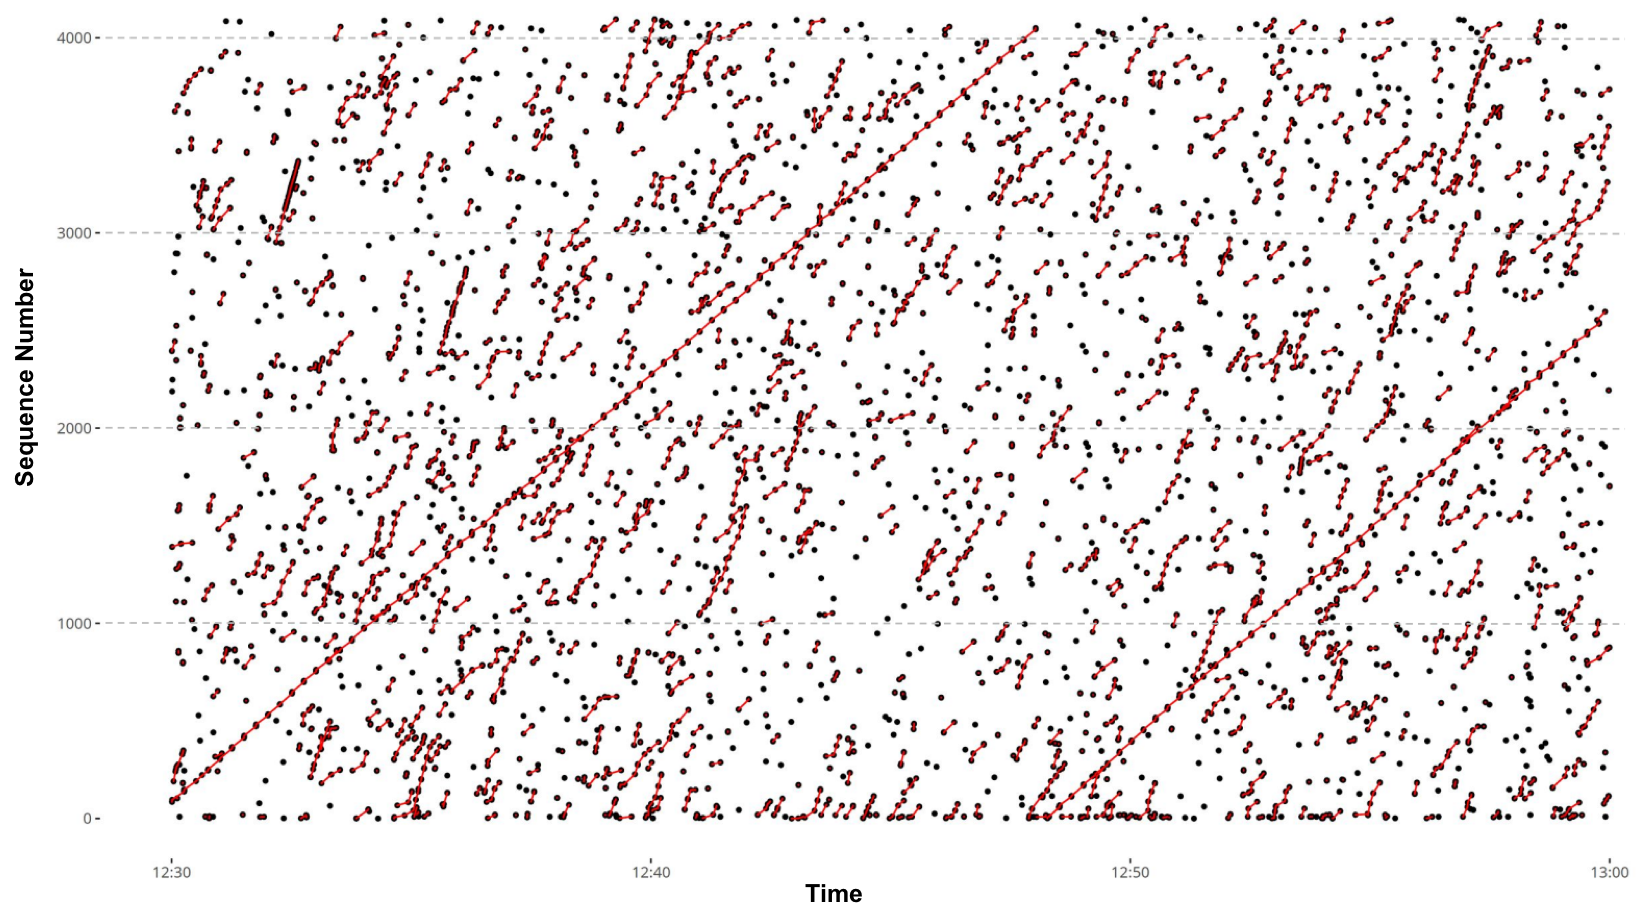
\includegraphics[width=0.8\textwidth]{outputs/clustering_1.png}
	  \caption{Clustering probe requests based on increasing sequence numbers generated over time.}
		\end{center}
	\end{figure*}

	There have been numerous attempts at using Wi-Fi
	to measure the volume and movement of people in built environment for various
	applications (\citep{zarim2006},\citep{sap2015},\citep{reki2007}).
	Though favorable results have been observed, one of the major 
	challanges been the changes in the MAC address randomisation process which 
	aims to protect the users' privacy by anonymising the only globally identifiable
	portion of the probe requests \citep{green2008}. There have been various 
	successful research in breaking this
	randomisation process to extract real MAC addresses \citep{martin2017}
	but this usually results in serious infringement on the user's
	privacy. There is a clear gap in the research for
	exploring methodologies with which we can estimate the
	number of unique mobile devices at a location without the need to fingerprint
	them using their MAC address which we try to address in this paper.

	The pilot survey was conducted on Oxford st. in London on 20 December 2017 from 12:30 to
	13:00. The data was collected parallely through two methods - Wi-Fi sensor and Android app.
	The Wi-Fi sensor collected all the probe requests broadcated around the area
	and recorded the timestamp at which they were colleted, MAC address of the source
	device anonymised using a hashing algorithm, organisationally unique identifier (OUI) of the
	vendor who manufactured the device, total length of the singal in bits, signal
	strength reported by the device in dBm, duration for which the signal was tranmmitted, 
	the service set identifier (SSID) to which the probe request has been sent to and the
	length of the extra tags in the packets. The android app recorded the timestamp
	of every touch on the screen by the surveyor which corresponds to a pedestrian 
	crossing a cordon on the sidewalk. 

	Approximately 60,000 probe requests were collected out of which   \% had
	randomised MAC addresses thus effectively anonymised.
	When we include these anonymised probe requests and count the number of unique
	devices present in dataset, we find that the difference between manual counting and sensor based counting
	is 425\% on average thus showing the need for using a different fingerprint other than MAC address for the
	anonymised probe requests. We first filter the data by removing all the probe requests reporting
	low signal strength. This classification is done using a kmeans - class interval algorithm.
	This reduces the difference from the manual count to 30\%.

	Then we turn our attention to other fields which can provide us information
	on the device which generated the probe request and hence enabling us to 
	finger print them uniquely.
	From a preliminary investigation, we find that the data fields - SSID and length of
	the tags are very sparse and not useful in identifying the unique device while 
	OUIs, length of the packet and sequence numbers can be crucial in doing the same.
	A pair of probes with the same OUI shows the device manufacturer and same length of the packet signifies that 
	there is a high probability that it was generated by a similar devcie.
	
	We first split the anonymised probe requests by the OUI and length then run a 
	graph based partition algorithm on them based on the sequence numbers. This 
	algortithm links probes with increasing sequence numbers in increasing time within a
	specific distance. It also enforces the rule that a probe request has only one 
	incoming and outgoing links. It then returns the membership of the probe requests in
	distinct connected clusters in the resulting graph thus classifying probe requests
	with sequentially increasing numbers as ones generated from the same device as shown in Figure 1. Finally
	all the individual subsets are joined and cleaned for repeating probe requests with
	unique clusters. This filtering in-turn reduces the difference of the sensor count to the manual count to 
	-18\%.

	The important detail to notice is that we have clustered and estimated unique device
	without the knowledge of the MAC address of the devices hence delivering output 
	without compromising the users' privacy. The methodology can be applications in 
	numerous footfall counting projects in retail, urban planning, facilities management etc.
	

	\printbibliography[title={References}]

\end{document}
